\section{Part 5: Heuristics in the Adaptive A*}
\label{sec: Part 5}

We now perform testing of \emph{Repeated Forward Adaptive $A_*$ search} and present the results compared to regular \emph{Repeated Forward $A^*$ search}. The difference with \emph{Adaptive $A^*$ search} is that after each call of the algorithm, we pass it new heuristic values which are updated based on the previous call to the function. By doing so, we are using previous knowledge and better guiding the algorithm in exploring new areas that are not known to lead to blockages.
\begin{figure}[H]
  \centering
  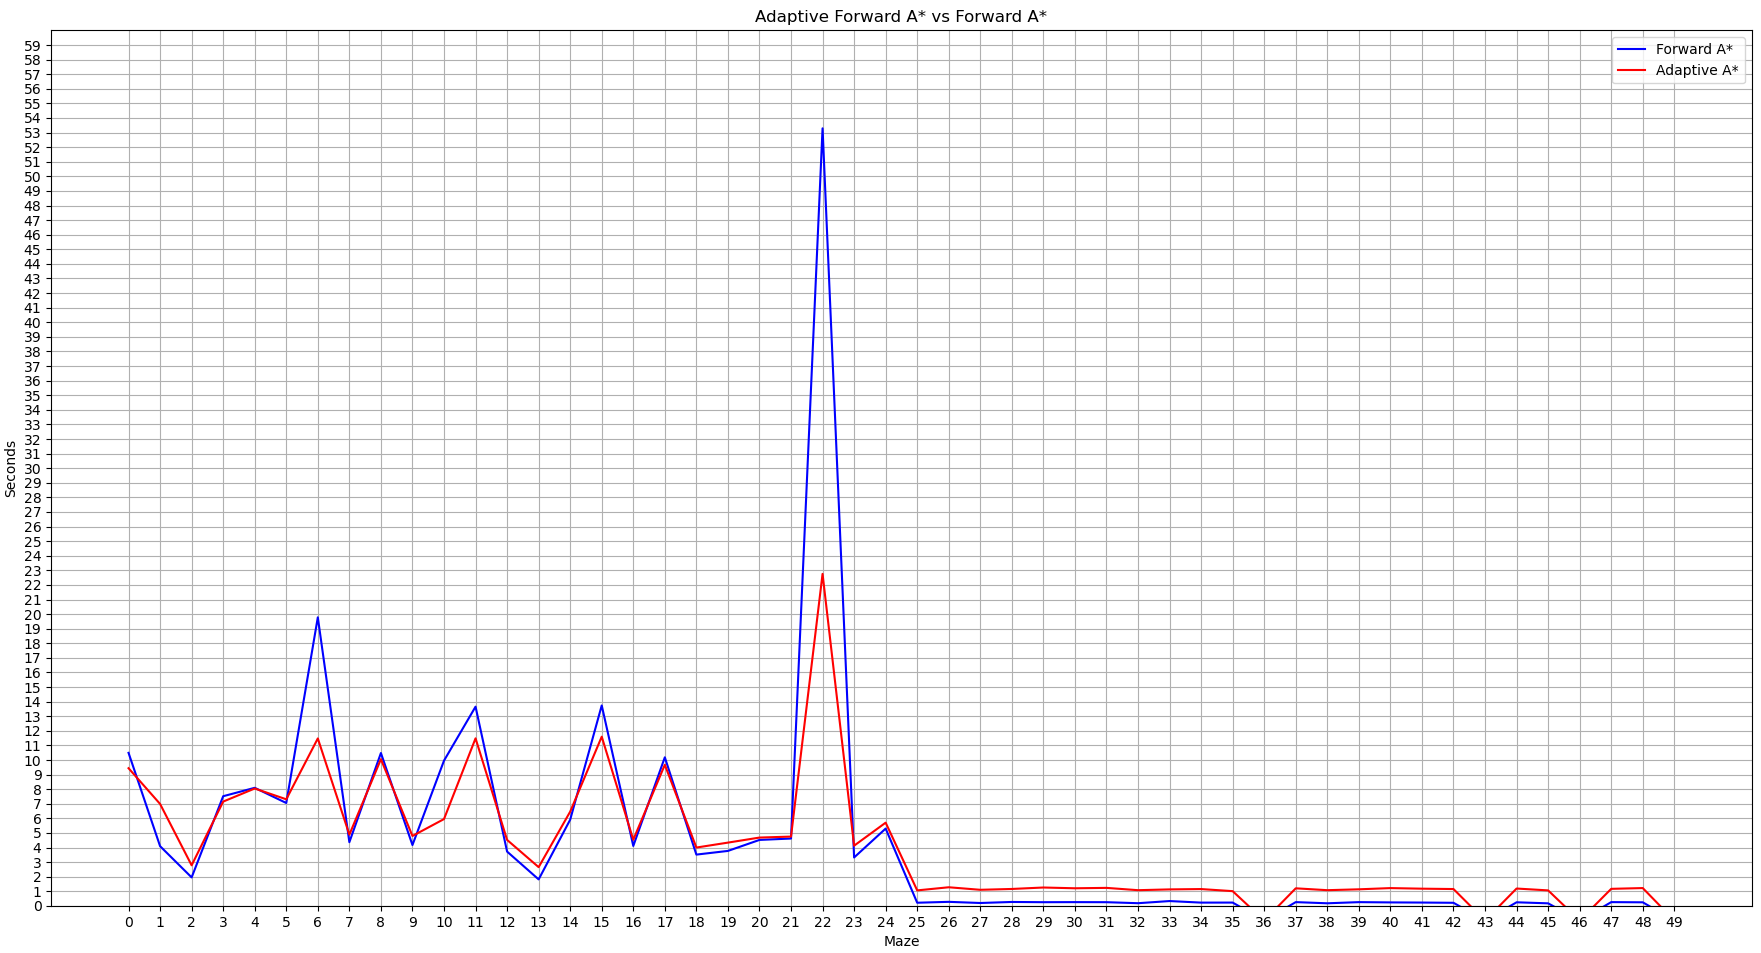
\includegraphics[width=1\linewidth]{Report/Part5/Figure_1.png}  
\caption{Repeated Adaptive Forward vs regular $A^*$ Comparison}
\end{figure}

Our results indicate that \emph{Adaptive $A^*$ search} does fair a bit better in complex mazes, such as our back tracked ones. However, we found that for simple random mazes, regular \emph{$A^*$ search} performs better. The reasoning for this is because in our random maze, each obstacle is usually simply overcome by going around the one or few walls, and a large alteration of the previous path is not needed. This means that by increasing the heuristics of previous expanded cells, we are forcing the algorithm to unnecessarily explore the surround areas first, rather than follow our classic depth first search method which regular $A^*$ performs. This is not a problem for our complex mazes because continuous walls exist. This means that most of the time, only one path exists and the agent is forced to move down a path. And updating the heuristics benefits the agent because at the few crossroads, where more than 1 path exists, the agent knows which path to take.